\documentclass[../main.tex]{subfiles}
%!TEX root = ./appendixFromAnalysisDossier.tex
\graphicspath {{../}}

\begin{document}
\section{Thruster Motor}
In order to determine the required torque of the servo that is at the end  of the thruster shaft, worst case scenario moments of inertia were considered, as seen in Figure \ref{fig:ThrusterI}. The angular acceleration can be set for any chosen servo motor as long as the acceleration is less than the specified maximum. The shaft could be either hollow or solid, therefore the solid case was chosen to account for the higher moment of inertia. The thruster motor and mounting bracket were considered as a single rectangular prism. The propeller was also considered as a rectangular prism.

\begin{equation}
T_{servo} = I_{total}\cdot{}\alpha
\end{equation}

\begin{equation}
I_{total} = \frac{m_{shaft}\cdot{}r_{st}^2}{2} + \frac{(m_{motor} + m_{bracket})}{12} \cdot{}(d_{m_{x}}^2 + d_{m_{z}}^2) + \frac{m_{prop}}{12}\cdot{}(d_{p+{x}}^2 + d_{p_{z}}^2)
\end{equation}

\begin{figure}[H]
	\centering
	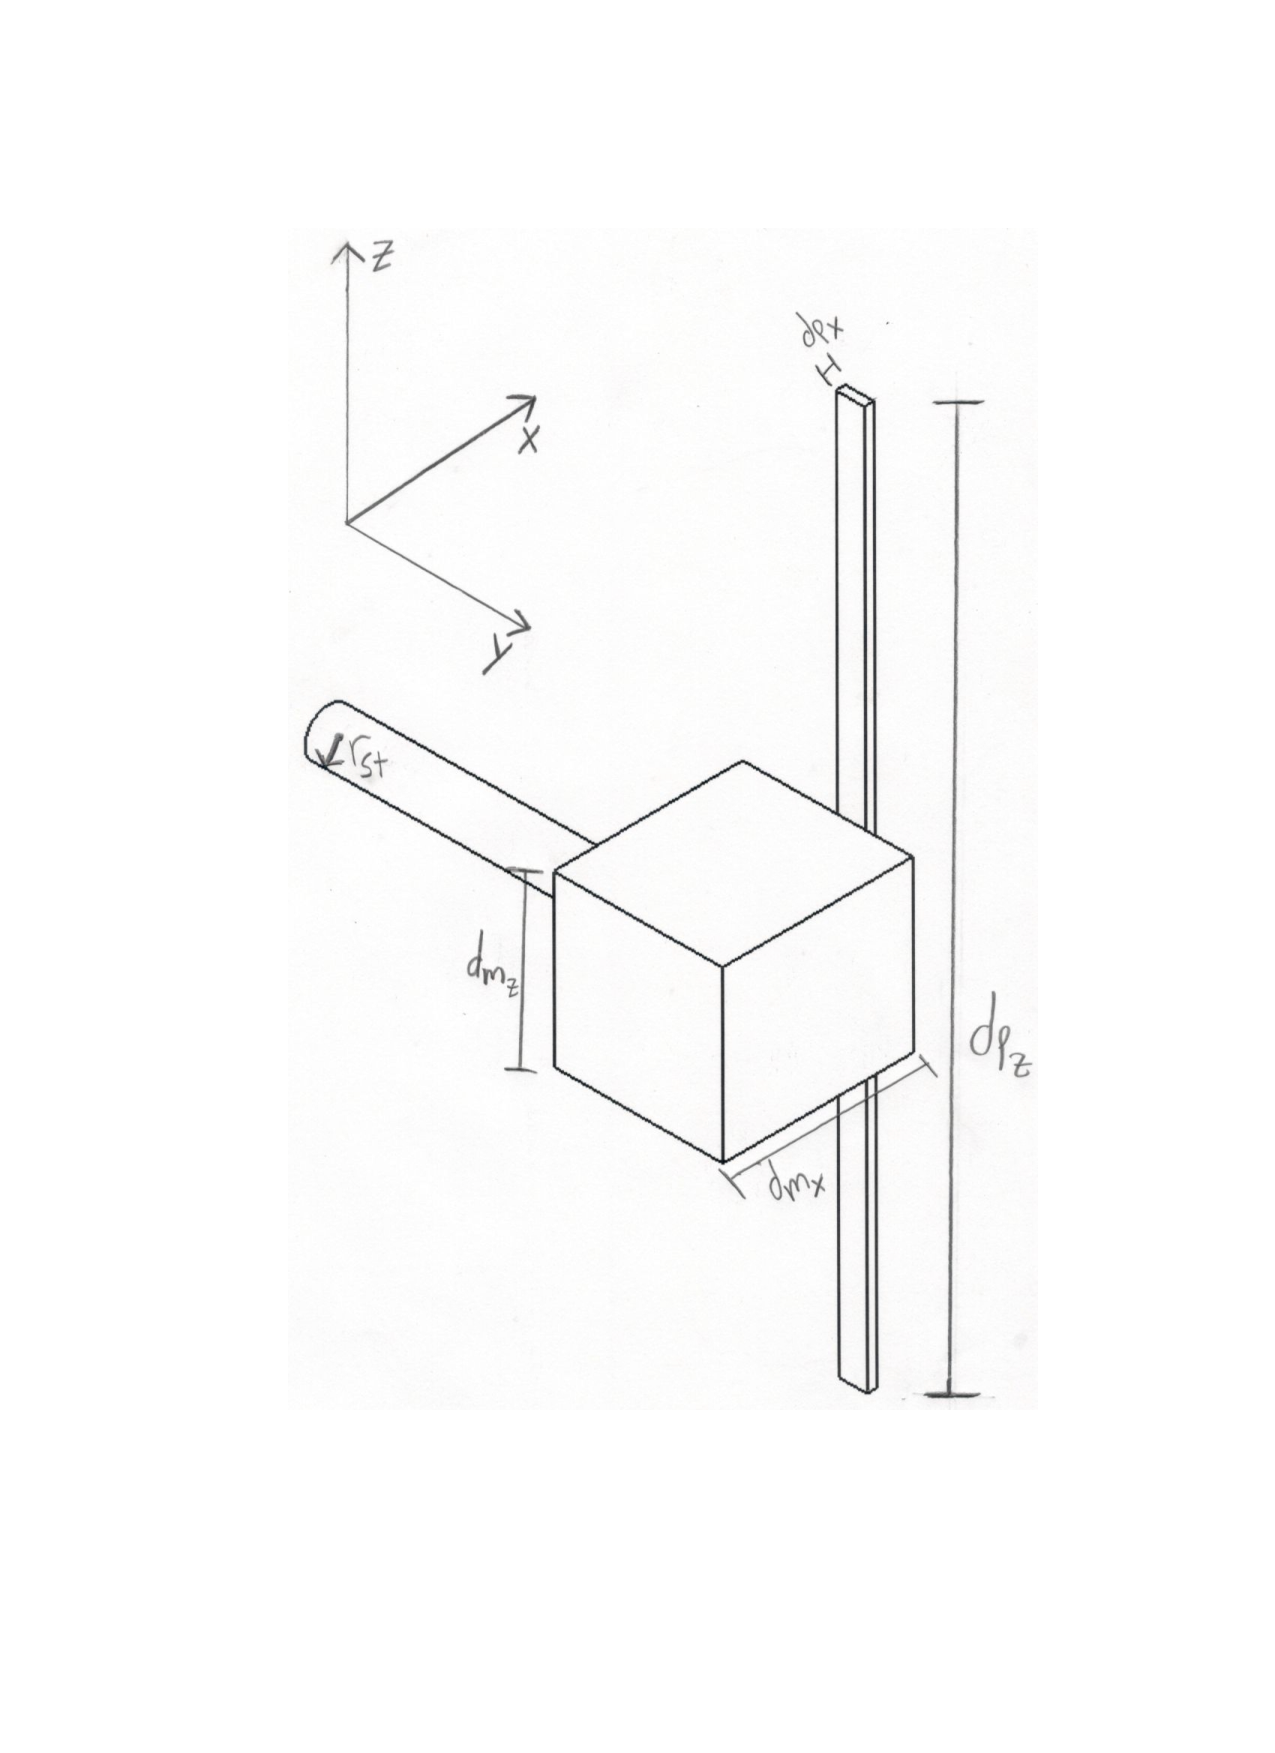
\includegraphics[width=0.5\textwidth]{img/analysis/thruster/thruster1.pdf}
	\caption{Thruster Pitching Shaft Worst Case Moment of Inertia}
	\label{fig:ThrusterI}
\end{figure}

\section{Thruster Bearing}
The bearing in the Bearing Shaft Support seen in Figure \ref{fig:ShaftLocation} will be mounted using a press fit. The calculations \cite{pressfit} for will need to be used for the bearing as the hub (shaft into bearing) and as the shaft (bearing into Bearing Shaft Support). These calculations assume similar materials for the hub and shaft.

\begin{figure}[H]
	\centering
	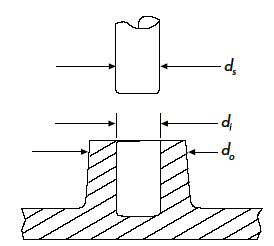
\includegraphics[width=0.5\textwidth]{img/analysis/thruster/pressfit.png}
	\caption{Pressfit Interference Diameters \cite{pressfit}}
	\label{fig:pressfit}
\end{figure}

\begin{equation}
\sigma_a=\frac{d_s-d_i}{d_s}\cdot{}E_p\cdot{}
\frac{d_o^2+d_s^2}{2d_o^2}
\end{equation}

\begin{equation}
i_a=d_s\cdot{}\frac{\sigma_a}{E_p}\cdot{}
\frac{d_o^2+d_s^2}{2d_o^2}
\end{equation}

\begin{equation}
n=\frac{S_y}{\sigma_a}
\end{equation}

\subsection{Sample Calculations}
Dimensions were taken from the first iteration of the design. Yield stress was estimated as 65MPa for the plastic parts.
 
\begin{equation*}
\sigma_a=\frac{6mm-(5.8mm)}{6mm}\cdot{}55MPa\cdot{}
\frac{(16mm)^2+(6mm)^2}{2(16mm)^2}=1.04MPa
\end{equation*}

\begin{equation*}
n=\frac{65MPa}{1.04MPa}=62.5
\end{equation*}

\begin{equation*}
i_a=(6mm)\cdot{}\frac{(1.04MPa)}{52.6MPa}\cdot{}
\frac{(16mm)^2+(6mm)^2}{2(16mm)^2}=0.068mm
\end{equation*}
	
\section{Gondola Hinge} \label{appendix:gondolaHinge}

The loading on the gondola hinge by forces $R_{x'}$ and $R_{z''}$ calculated in system modelling section \ref{gondola2ref} will be relatively small. Stress concentration would occur at points A and B shown in Figure \ref{fig:fillethinge}, however to avoid these stress concentrations fillets will be added to the part. 

\begin{figure}[H]
	\centering
	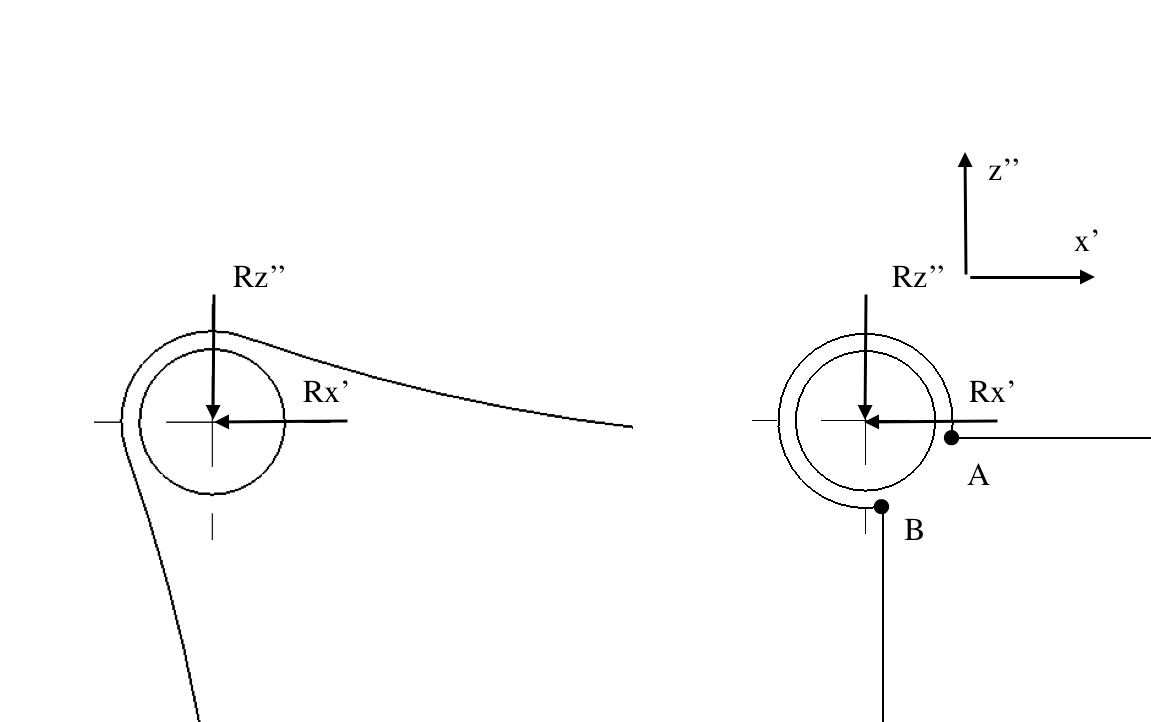
\includegraphics[width=1\textwidth]{img/gondola/filletHinge.PNG}
	\caption{Gondola Hinge Comparison Fillet Vs. No Fillet}
	\label{fig:fillethinge}
\end{figure}

The hinge pin will likely be made of aluminium and the shear stress experienced by the part will not be considerable relative to the strength of the material. 

\end{document}